\subsection{MobileNetV2: Inverted Residuals and Linear Bottlenecks}

Originally introduced as MobileNet by Howard \etal~\cite{MobileNet}, the idea
was to bring powerful computer vision models to embedded systems, by offering
state-of-the-art performance at greatly decreased computational cost. MobileNet
presented a novel idea in the way convolution layers work, by using depthwise
separable filters, which factorize a convolution into a depthwise convolution
-- acting on each channel independently -- and a pointwise convolution
(essentially a $1\times1$ convolution to combine each depthwise convolution).\\

Building upon this idea, Sandler \etal~\cite{MobileNetV2} presented
MobileNetV2, which utilizes inverted residuals between narrow layers where
linearity is preserved (as to maintain the representational power), while still
exploiting depthwise convolutions to introduce non-linearity in the
intermediate layers.

The peculiarity of depthwise filters is not in their performance, since they
achieve a somewhat similar result to traditional convolution filters for
feature extraction, but rather in their astounding efficiency, reducing
computation by a factor of almost $k^2$~\cite{MobileNetV2}.

Furthermore, the model is easily adaptable to multiple problems, and offers
several choices for any application's needs in terms of accuracy versus
performance ratio, by providing a width multiplier parameter, $\alpha$, which
reduces or enlarges the input and output channels of each layer by a factor of
$\alpha$ (except for the last convolution layer for the case of MobileNetV2).
This has the potential to greatly reduce the amount of trainable parameters,
and in turn decreases the computational cost, if set to a value below 1.\\

It goes without saying that such trade-off between accuracy and efficiency is a
perfect match for an embedded object detection network, aimed to run on a
drone, since the model still outperforms state-of-the-art Single Shot Detectors
on the COCO dataset~\cite{MobileNetV2}.

\begin{figure}[h]
	\centering
	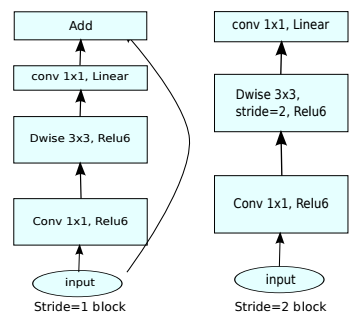
\includegraphics[width=0.45\textwidth]{figure/mobilenetv2.png}
	\caption{MobileNetV2: Inverted residuals}
	\label{fig:invertedresiduals}
\end{figure}

\subsubsection{Modifications}

Similarly to DroNet, the output layer uses the softmax activation function, as
well as a categorical cross-entropy loss function along with the Adam optimizer
with its default hyper parameters.

As for the input layer, since MobileNetV2 was originally trained on the
ImageNet dataset, it was intended to use $224\times224\times3$ images. However,
the image format used in this work is $340\times255\times C$ (as explained in
the last section), therefore the fully convolution layer at the top of the
network is not included, but the rest of the network uses the original weights
by transfer learning.

More modifications to the final layers of the network are added later on for
experimentation, and are explained in due time.
